\chapter{Desarrollo del proyecto}

\section{Planteamiento}

\section{Planificaci�n del proyecto}

\section{Tecnolog�as empleadas en el proyecto}

\section{Herramientas utilizadas en el proyecto}

\section{Hardware}
En esta parte se explica detalladamente el hardware empleado en el desarrollo del proyecto.

\subsection{Pioneer 3 AT}

El robot Pioneer 3 AT (Figura \ref{fig:pioneer3at}), perteneciente a la empresa Adept MobileRobots, es un robot de cuatro ruedas en configuraci�n skid-steer y todo terreno (AT, All Terrain) de operaci�n e investigaci�n en laboratorio.\\

\begin{figure}[htp]
\centering
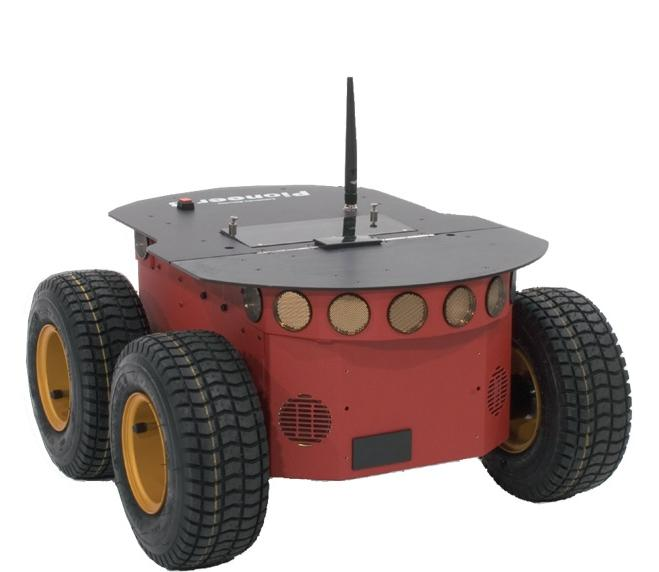
\includegraphics[width=0.4\textwidth]{figuras/pioneer_3_at.jpg}
\caption{Robot Pioneer 3-AT} \label{fig:pioneer3at}
\end{figure}

Su configuraci�n en skid-steer permite un control relativamente simple utilizando el modo diferencial para poder realizar giros con gran maniobrabilidad, sin embargo, esta configuraci�n depende mucho del tipo de suelo, con lo que se pierde precisi�n.\\

Este robot dispone de bater�as, interruptor con parada de emergencia, dos motores de corriente continua para cada par de ruedas con transmisi�n mediante correa, encoders para leer la odometr�a y un microcontrolador con firmware ARCOS.\\

Ademas cuenta con un peque�o computador interno conectado al microcontrolador que puede utilizarse para realizar operaciones de manera aut�noma.\\

El cuerpo del robot es de aluminio y su parte delantera as� como superior es f�cilmente desmontable para realizar las conexiones pertinentes y acceder al ordenador de a bordo y la placa microcontroladora. En la plataforma superior se sit�a el panel de control (Figura \ref{fig:panel_control})para acceder al ordenador de abordo conectando un monitor, teclado y rat�n, puerto serial RS-232, botones de encendido y reset varios leds indicadores de estado y de env�o y recepci�n de datos.\\

\begin{figure}[htp]
\centering
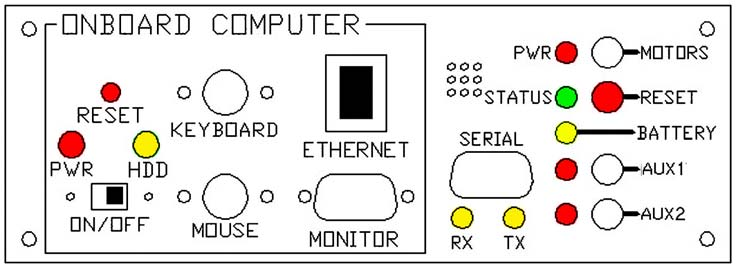
\includegraphics[width=0.6\textwidth]{figuras/panel_control.png}
\caption{Panel de control del robot Pioneer 3-AT} \label{fig:panel_control}
\end{figure}

En la siguiente tabla se describen las principales caracter�sticas del robot.\\

% Please add the following required packages to your document preamble:
% \usepackage{graphicx}
\begin{table}[!h]
\centering
\resizebox{\textwidth}{!}{%
\begin{tabular}{c c}
\hline
{\bf Especificaciones} & {\bf Pioneer 3 AT} \\ \hline
Largo & 508 mm \\
Ancho & 497 mm \\
Alto & 277 mm \\
Distancia al suelo & 80 mm \\
Peso & 12 kg \\
Carga �til & 32 kg \\
Cuerpo & Aluminio de 1.6 mm \\
Bater�as & 3 de 12 V ~Ah, estancas, plomo-�cido \\
Autonom�a & 4-8 horas \\
Sistema motriz & 4 ruedas motrices \\
Ruedas & Neum�ticos de Nylon \\
Di�metro de rueda & 222 mm \\
Ancho de rueda & 88 mm \\
Sistema de giro & Diferencial \\
radio m�xima curvatura & 40 cm \\
Radio de giro & 0 cm \\
M�xima velocidad de avance & 1.2 m/s \\
M�ximo escal�n & 10 cm \\
M�ximo hueco & 15.2 cm \\
Terreno & Asfalto, Tierra, C�sped, etc. \\
Encoders & 500 pulsos \\
Procesador & Hitachi H8S \\ \hline
\end{tabular}
}
\caption{Especificaciones del robot Pioneer 3 AT}
\label{my-label}
\end{table}


\subsection{Sensor Kinect}



\subsection{L�ser SICK LMS100}
